\documentclass{article}
\setlength{\parskip}{5pt} % esp. entre parrafos
\setlength{\parindent}{0pt} % esp. al inicio de un parrafo
\usepackage{amsmath} % mates
\usepackage[sort&compress,numbers]{natbib} % referencias
\usepackage{url} % que las URLs se vean lindos
\usepackage[top=25mm,left=20mm,right=20mm,bottom=25mm]{geometry} % margenes
\usepackage{hyperref} % ligas de URLs
\usepackage{graphicx} % poner figuras
\usepackage[spanish]{babel} % otros idiomas
\usepackage[utf8]{inputenc}
\usepackage{wrapfig}
\usepackage{listings}
\usepackage{xcolor}
\usepackage{subfig} 
\definecolor{codegreen}{rgb}{0,0.6,0}
\definecolor{codegray}{rgb}{0.5,0.5,0.5}
\definecolor{codepurple}{rgb}{0.58,0,0.82}
\definecolor{backcolour}{rgb}{0.95,0.95,0.92}
 
\lstdefinestyle{mystyle}{
    backgroundcolor=\color{backcolour},   
    commentstyle=\color{codegreen},
    keywordstyle=\color{magenta},
    numberstyle=\tiny\color{codegray},
    stringstyle=\color{codepurple},
    basicstyle=\footnotesize,
    breakatwhitespace=false,         
    breaklines=true,                 
    captionpos=b,                    
    keepspaces=true,                 
    numbers=left,                    
    numbersep=5pt,                  
    showspaces=false,                
    showstringspaces=false,
    showtabs=false,                  
    tabsize=2
}
\lstset{style=mystyle}
\lstset{language=Python}
\author{Equipo 4 \\Jorge  Fuentes, Tania  Hernandez,
 Anahi Herrera, Gustavo  Díaz, Miriam  Mata, Alejandro Ramos} % author
\title{Práctica 3 \\ Diseño de la estructura de un panorámico} % titulo
\date{\today}

\begin{document} % inicia contenido
\maketitle % cabecera
\begin{abstract} % resumen
\textbf{Objetivo:} El estudiante deberá presentar una propuesta de análisis de formas y de la programación para la ejecución de la optimización (descripción funcional) de características de trabajo especificas que presenta la(s) ventaja(s) (mencionar ventajas). La Forma de una obra, se refiere a la manera como está escrita, cómo es por fuera, de qué manera se proyectan las ideas de su contenido. El comentario de formas artísticas está sujeto, básicamente, al estudio de un conjunto de aspectos de carácter formal y estilístico, pero no debe analizarse la obra sin tomar en cuenta el contexto histórico y cultural en el que dicha obra artística se produce. Proceso de separación de las partes de un determinado elemento para estudiar su función, significado y naturaleza.\\
\end{abstract}
\newpage
\tableofcontents
\newpage
\section{Introducción}\label{intro} % seccion y etiqueta
El análisis formal de conceptos estudia las relaciones existentes en conjuntos de datos y revela las estructuras de los mismos. La Forma de una obra, se refiere a la manera como está escrita, cómo es por fuera, de qué manera se proyectan las ideas de su contenido. El comentario de formas artísticas está sujeto, básicamente, al estudio de un conjunto de aspectos de carácter formal y estilístico, pero no debe analizarse la obra sin tomar en cuenta el contexto histórico y cultural en el que dicha obra artística se produce. Proceso de separación de las partes de un determinado elemento para estudiar su función, significado y naturaleza\cite{rf1}. Al analizarlas en una obra pueden ser formales, es decir, que se ven, como las líneas de contorno, o las que se usan para crear texturas, o informales, las que se intuyen, que indican direcciones o sensaciones espaciales de profundidad u otras. Analizar la forma de los objetos no consiste solo en mirarlos, hay que “saber” verlos. Todo dibujante antes de comenzar un trabajo, debe observar detenidamente el modelo, buscando en él proporciones semejantes, puntos alineados entre otros, es decir, debe recurrir a pequeñas ayudas que le faciliten la comprensión en conjunto de la del modelo. Esta práctica, que es inusual en otro tipo de actividades, resulta de una enorme utilidad en la ejecución de dibujos. En los ejemplos que se ven a continuación se desarrollan de forma didáctica estos conceptos que no todo dibujante debe tener en cuenta antes de representar un modelo.
%\cite{ff2} CITAR FUENTE

%\begin{figure} % figura
    %\centering
    %\includegraphics[width=150mm]{output3.jpg} % archivo
    %\caption{resultados del programa}
    %\label{grafica}
%\end{figure}
\section{Desarrollo}
\subsection{Nombre y definición de la forma geometría}
\subsubsection{Estructura de un panorámico}
Este tipo de estructura aparentemente es muy sencilla porque cuenta solamente con tres partes principales que son: la mampara, el pedestal y la cimentación; en la Figura 1 se muestran esquemáticamente estas tres partes. Sin embargo, vista en forma minuciosa, una mampara consta de varios componentes y accesorios que hacen que esta estructura sea realmente muy compleja tanto en su diseño estructural, como en su construcción y también en su comportamiento sobre todo ante viento como el producido por huracán o tromba. Tanto la cimentación como el pedestal y la mampara elevada pueden constar de diversos elementos tales como: anclas suelo–zapata, vigas estabilizadoras, anclas pedestal–zapata, lastres, placas-base, acartelamientos, el tubo del pedestal, escaleras externas e internas, andamios, placas de conexión pedestal-mampara, travesaño principal de la mampara, placas verticales del travesaño, armaduras, pernos de sujeción, láminas de la mampara, accesorios de iluminación, ganchos o argollas de sujeción, travesaños secundarios; además, se tienen diversos elementos de sujeción o conexión tales como pernos, tornillos, remaches, soldaduras, etc\cite{rf2}.
\begin{figure}[!tbp]
  \centering
  \subfloat[]{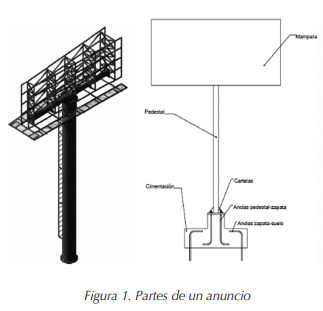
\includegraphics[width=0.4\textwidth]{Imagen1.png}\label{fig:f1}}
  \hfill
  \subfloat[]{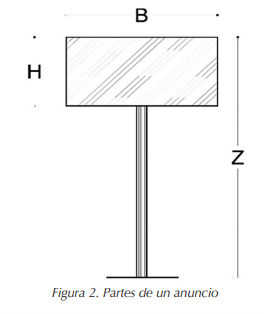
\includegraphics[width=0.4\textwidth]{Imagen2.png}\label{fig:f2}}
  \caption{Panorámico}
\end{figure}
\newpage
\subsection{Estado del arte}
Este tipo de estructura aparentemente es muy sencilla porque cuenta solamente con tres partes principales que son: la mampara, el pedestal y la cimentación; en la Figura 1 se muestran esquemáticamente estas tres partes. Sin embargo, vista en forma minuciosa, una mampara consta de varios componentes y accesorios que hacen que esta estructura sea realmente muy compleja tanto en su diseño estructural, como en su construcción y también en su comportamiento sobre todo ante viento como el producido por huracán o tromba\cite{rf3}. Tanto la cimentación como el pedestal y la mampara elevada pueden constar de diversos elementos tales como: anclas suelo–zapata, vigas estabilizadoras, anclas pedestal–zapata, lastres, placas-base, acartelamientos, el tubo del pedestal, escaleras externas e internas, andamios, placas de conexión pedestal-mampara, travesaño principal de la mampara, placas verticales del travesaño, armaduras, pernos de sujeción, láminas de la mampara, accesorios de iluminación, ganchos o argollas de sujeción, travesaños secundarios; además, se tienen diversos elementos de sujeción o conexión tales como pernos, tornillos, remaches, soldaduras, etc.
\newpage
\subsection{Pasos del desarrollo de la programación}
A continuación, veremos la codificación de la programación en MATLAB.
\begin{lstlisting}
%%%% A 99 LINE TOPOLOGY OPTIMIZATION CODE BY OLESIGMUND, OCTOBER 1999 %%%
function topp3(nelx,nely,volfrac,penal,rmin);
% INITIALIZE
x(1:nely,1:nelx) = volfrac;
loop = 0;
%Declarando vacio
for ely = 1:nely
 for elx = 1:nelx
 if (((ely-(nely*0.5)<(2*elx)-(1.36*nelx)) |(ely <(1+nely*0.5))) &(elx >(1+nelx)*0.6666))
 passive(ely,elx) = 1;
 else
 passive(ely,elx) = 0;
 end
 end
end
x(find(passive))=0.001;
change = 1.;
% START ITERATION
while change > 0.01
loop = loop + 1;
xold = x;
% FE-ANALYSIS
 [U]=FE(nelx,nely,x,penal);
%13 OBJECTIVE FUNCTION AND SENSITIVITY ANALYSIS
 [KE] = lk;
 c = 0.;
 for ely = 1:nely
 for elx = 1:nelx
 n1 = (nely+1)*(elx-1)+ely;
 n2 = (nely+1)* elx +ely; %19
 dc(ely,elx) = 0.;
 for i = 1:5
 Ue = U([2*n1-1;2*n1; 2*n2-1;2*n2; 2*n2+1; 2*n2+2;
2*n1+1;2*n1+2],1);
 c = c + x(ely,elx)^penal*Ue'*KE*Ue;
 dc(ely,elx) = dc(ely,elx)-penal*x(ely,elx)^(penal-1)*Ue'*KE*Ue;
 end
 end
end
%25 FILTERING OF SENSITIVITIES
[dc] = check(nelx,nely,rmin,x,dc);
%27 DESIGN UPDATE BY THE OPTIMALITY CRITERIA METHOD
[x] = OC(nelx,nely,x,volfrac,dc,passive);
%29 PRINT RESULTS
change = max(max(abs(x-xold)));
disp(['It.:' sprintf('%4i',loop) 'Obj.:' sprintf('%10.4f',c) ...
' Vol.: ' sprintf('%6.3f',sum(sum(x))/(nelx*nely)) ...
' ch.: ' sprintf('%6.3f',change )])
% PLOT DENSITIES
colormap(gray); imagesc(-x); axis equal; axis tight; axis off;pause(1e6);
end
%40 %%%%%%%%% OPTIMALITY CRITERIA UPDATE %%%%%%%%%
function [xnew]=OC(nelx,nely,x,volfrac,dc,passive)
l1 = 0; l2 = 100000; move = 0.2;
while (l2-l1 > 1e-4)
lmid = 0.5*(l2+l1);
xnew = max(0.001,max(x-move,min(1.,min(x+move,x.*sqrt(-dc./lmid)))));
xnew(find(passive)) = 0.001;
if sum(sum(xnew)) - volfrac*nelx*nely > 0;
l1 = lmid;
else
l2 = lmid;
end
end
%%%%%%%%%% MESH-INDEPENDENCY FILTER %%%%%%%%%%%
function [dcn]=check(nelx,nely,rmin,x,dc)
dcn=zeros(nely,nelx);
for i = 1:nelx
for j = 1:nely
sum=0.0;
for k = max(i-round(rmin),1):min(i+round(rmin),nelx)
for l = max(j-round(rmin),1):min(j+round(rmin), nely)
fac = rmin-sqrt((i-k)^2+(j-l)^2);
sum = sum+max(0,fac);
dcn(j,i) = dcn(j,i) + max(0,fac)*x(l,k)*dc(l,k);
end
end
dcn(j,i) = dcn(j,i)/(x(j,i)*sum);
end
end
%65 %%%%%%%%% FE-ANALYSIS %%%%%%%%%%%%
function [U]=FE(nelx,nely,x,penal)
[KE] = lk;
K = sparse(2*(nelx+1)*(nely+1), 2*(nelx+1)*(nely+1));
F = sparse(2*(nely+1)*(nelx+1),5); U =zeros(2*(nely+1)*(nelx+1),5);
for ely = 1:nely
for elx = 1:nelx
n1 = (nely+1)*(elx-1)+ely;
n2 = (nely+1)* elx +ely;
edof = [2*n1-1; 2*n1; 2*n2-1; 2*n2; 2*n2+1;2*n2+2;2*n1+1; 2*n1+2];
K(edof,edof) = K(edof,edof) + x(ely,elx)^penal*KE;
end
end
% DEFINE LOADSAND SUPPORTS(HALF MBB-BEAM)
F(2*nelx*(nely+1)+2,1) = 1;
F(2*nelx*(nely+1)+(nely/4),2) = 1;
F(2*nelx*(nely+1)+(nely/2),3) = 1;
F(2*nelx*(nely+1)+(nely),4) = 1;
F(2*nelx*(nely+1)+(nely*1.2),5) = 1;
fixeddofs =2*(nely+1):2*(nely+1):2*(nelx+1)*(nely+1);
alldofs = [1:2*(nely+1)*(nelx+1)];
freedofs = setdiff(alldofs,fixeddofs);
% SOLVING 127
U(freedofs,:) = K(freedofs,freedofs) \F(freedofs,:);
U(fixeddofs,:)= 0;
%%%%%%%%%% ELEMENT STIFFNESS MATRIX %%%%%%%
function [KE]=lk
E = 1.;
nu = 0.3;
k=[ 1/2-nu/6 1/8+nu/8 -1/4-nu/12 -1/8+3*nu/8 ...
-1/4+nu/12 -1/8-nu/8 nu/6 1/8-3*nu/8];
KE = E/(1-nu^2)*[ k(1) k(2) k(3) k(4) k(5) k(6) k(7) k(8)
k(2) k(1) k(8) k(7) k(6) k(5) k(4) k(3)
k(3) k(8) k(1) k(6) k(7) k(4) k(5) k(2)
k(4) k(7) k(6) k(1) k(8) k(3) k(2) k(5)
k(5) k(6) k(7) k(8) k(1) k(2) k(3) k(4)
k(6) k(5) k(4) k(3) k(2) k(1) k(8) k(7)
k(7) k(4) k(5) k(2) k(3) k(8) k(1) k(6)
k(8) k(3) k(2) k(5) k(4) k(7) k(6) k(1)];
\end{lstlisting}
\begin{figure}[htp] % figura
    \centering
    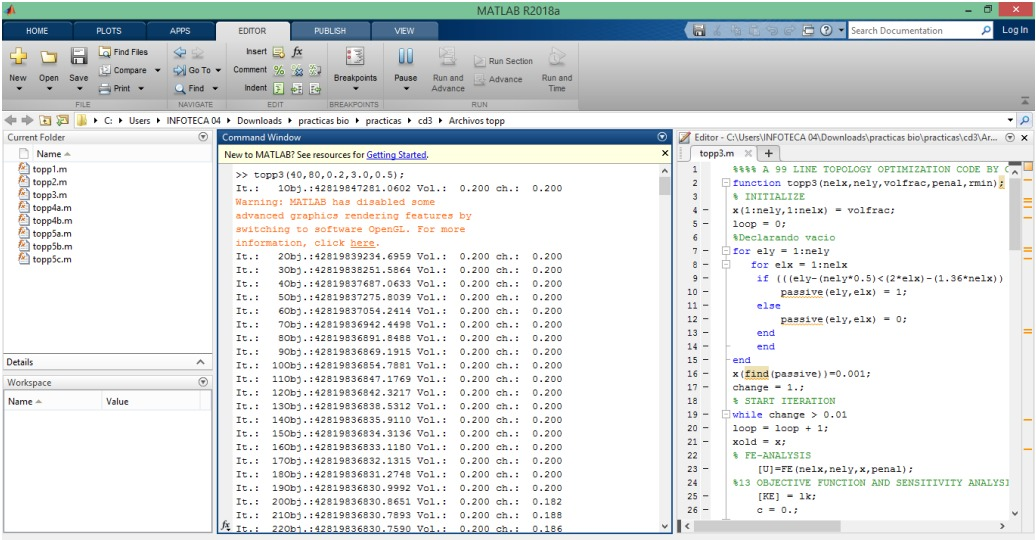
\includegraphics[width=125mm]{Resultado.jpeg} % archivo
    \caption{Configuraciones iniciales y análisis.}
    \label{grafica}
\end{figure}
\newpage
\subsection{Resultados de la optimización}
\begin{figure}[htp] % figura
    \centering
    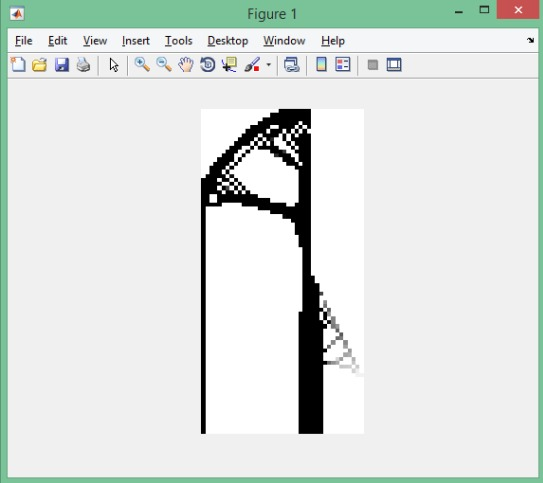
\includegraphics[width=100mm]{Optimizacion.jpeg} % archivo
    \caption{Resultado.}
    \label{grafica}
\end{figure}
\begin{figure}[htp] % figura
    \centering
    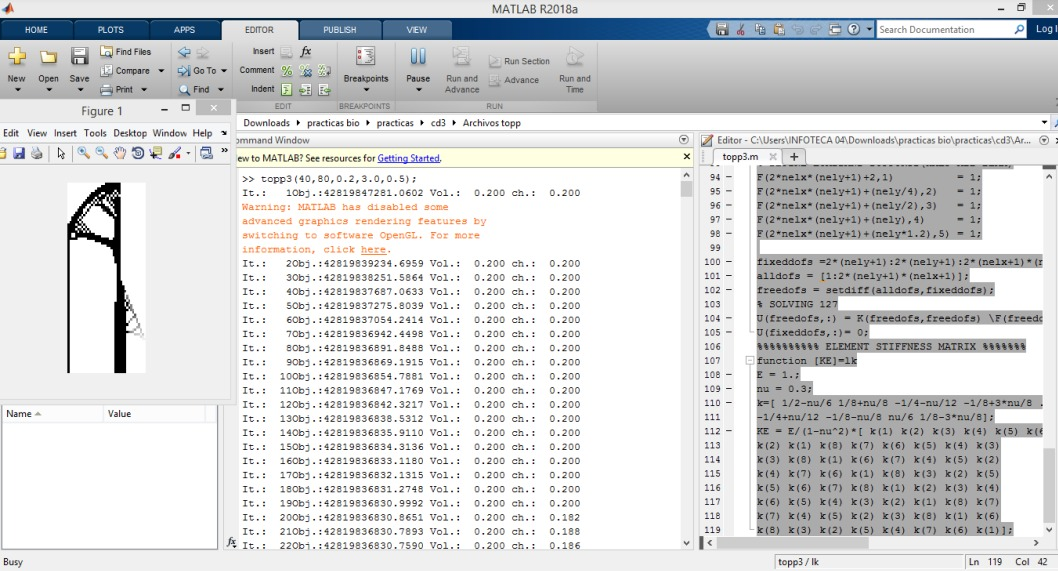
\includegraphics[width=150mm]{Ejemplo Completo.jpeg} % archivo
    \caption{Vista completa del resultado.}
    \label{grafica}
\end{figure}
 \newpage
\section{Conclusiones}
\subsection{Jorge  Fuentes}
En esta ocasión tratando de cumplir el objetivo planteado de presentar una propuesta de análisis de formas y de la programación para la ejecución de la optimización de características de trabajo especificas que presenta las ventajas ahora en esta práctica 3 sobre el diseño de la estructura de un panorámico, aplicando los conocimientos previos sobre nuestro dominio en MATLAB así como los pasos de la programación logramos elaborar una estructura de la base de un panorámico.
\subsection{Tania  Hernandez}
La práctica realizada consistió en la elaboración de la estructura de un panorámico, para la cual como en todas las anteriores prácticas, se buscó la información respecto a su forma geométrica, estado del arte, etc. Para así pasarnos al resultado final, el cual es la estructura del panorámico ya finalizada.
\subsection{Anahi Herrera}
Gracias a la elaboración de esta práctica se entendió de una mejor manera el funcionamiento de MATLAB aplicado hacia la materia de biomecánica, se realizaron investigaciones grupales llevando esta teoría recopilada a la práctica de manera exitosa. 
\newpage
\subsection{Gustavo  Díaz}
Al nosotros conocer un poco mas sobre el funcionamiento de un panorámico/espectacular es más sencillo poder comprender el cómo están hechos para su correcto funcionamiento dado que al ser una estructura que solo se encuentra en soportado por lo que se podría decir un solo punto todas las fuerzas que se genera por sí solo el panorámico y las que se generan por parte de las inclemencias del tiempo hacen que una estructura tan grande tenga diferentes tipos de soportes interiores o externos que lo ayuden a soportar el peso al nosotros hacer la simulación pudimos ver donde es que se concentran la mayoría de los esfuerzos que recaen sobre la estructura y pudimos ver la manera de mejorarla por medio de la optimización.
\subsection{Miriam  Mata}
Esta práctica fue mas complicada que las pasadas mas que nada por el matlab pero se concluyó con éxito la práctica, con cada práctica que vamos realizando siento que vamos desarrollándonos más en el área de programación aunque sea solo en Matlab, muchos de los lenguajes son muy parecidos y así en un futuro se nos haría más fácil realizar códigos aunque sea en otros lenguajes.
\subsection{Alejandro Ramos}
En esta práctica lo que hicimos fue una estructura que fue de un panorámico lo más interesante fue ver el resultado de nuestro trabajo nos quedó excelente, también me pareció muy importante el saber analizar las formas y que no cualquiera lo puede hacer de buena manera debido a que se debe saber analizarlas para hacerlo bien espero seguir aprendiendo más en las siguientes prácticas.
\bibliography{bib}
\bibliographystyle{plainnat}
\end{document}
